\documentclass[11pt]{article}
\usepackage{amsmath, amsthm, epsfig, amsfonts, amssymb, listings, enumerate, color, hyperref, mdframed}
\usepackage[utf8]{inputenc}
\usepackage[T1]{fontenc}
\usepackage{lmodern}
\usepackage[french]{babel}

\usepackage{fancyhdr}
\usepackage{lastpage}

\pagestyle{fancy}
\lhead{Programmation en C}
\chead{}
\rhead{EPFL -- Automne 2017}
\headsep = 24pt
\fancyfoot{}
\rfoot{\thepage\ / \pageref{LastPage}}
\renewcommand{\headrule}{\vbox to 0pt{\hbox to \headwidth{\dotfill}\vss}}
\fancyhfoffset[H]{0pt}
\renewcommand{\footrulewidth}{0pt}

\definecolor{dkgreen}{rgb}{0,0.6,0}
\definecolor{gray}{rgb}{0.5,0.5,0.5}
\definecolor{mauve}{rgb}{0.58,0,0.82}

\definecolor{mygray}{rgb}{0.4,0.4,0.4}
\definecolor{mygreen}{rgb}{0,0.8,0.6}
\definecolor{myorange}{rgb}{1.0,0.4,0}
\lstset{frame=tblr,
  language=[ANSI]C,
  aboveskip=3mm,
  belowskip=3mm,
  showstringspaces=false,
  columns=flexible,
  basicstyle={\small\ttfamily},
%  numbers=left,
  numberstyle=\tiny\color{gray},
  keywordstyle=\color{blue},
  commentstyle=\color{dkgreen},
  stringstyle=\color{mauve},
  breaklines=true,
  breakatwhitespace=true
  tabsize=3
}

\textheight 23cm
\textwidth 16.5cm
\voffset -2.5cm
\hoffset -2cm

\parindent 0cm
\parskip.5\baselineskip

\begin{document}

%========================
\begin{center}{\bf Session d'exercices -- Structures et pointeurs}\\
\textbf{\emph{Echantillonage}}
\end{center}

En traitement du signal, on sait qu'un signal échantilloné a une certaine fréquence d'échantillonage peut être parfaitement reconstruit si la fréquence du signal est strictement inférieure à la moitié de la fréquence d'échantillonage. On appelle cette fréquence maximale la fréquence de Nyquist. Dans cet exercice, nous définirons deux structures représentant les caractéristiques d'un signal sinusoïdal simple et d'un échantillonage et utiliserons ensuite ces structures pour vérifier la théorie en échantillonant des signaux de fréquences diverses. A noter que dans cet exercice, un signal complet est défini comme étant une somme de signaux sinusoïdaux.\\
\\
Si la théorie sous-jacente n'est plus très claire pour vous, vous trouverez des informations sur les pages suivantes : 
\begin{itemize}
\item Signaux sinusoïdes : https://fr.wikipedia.org/wiki/Signal_sinuso%C3%AFdal
\item Echantillonage : https://fr.wikipedia.org/wiki/%C3%89chantillonnage_(signal)
\item Théorème d'échantillonage : https://fr.wikipedia.org/wiki/Th%C3%A9or%C3%A8me_d%27%C3%A9chantillonnage 
\end{itemize}

\begin{enumerate}[a)]

\item \textcolor{mygreen}{[Difficulté: *]}
Ecrivez la structure
\begin{center}
\texttt{Sinusoide}, 
\end{center}
qui doit contenir 3 champs représentant les 3 constantes inhérentes d'un signal sinusoïdal pur : la fréquence, l'amplitude et le déphasage.

\item \textcolor{mygreen}{[Difficulté: *]}
Écrivez la structure
\begin{center} 
\texttt{Echantillonage}, 
\end{center}
qui doit contenir 2 champs représentant l'instant auquel l'échantillonage commence et sa fréquence.

\vspace{20pt}
\hspace{-20pt} Continuez en écrivant tout ce qui manque pour compléter le programme, incluant ce qui suit :
\vspace{20pt}

\item \textcolor{mygreen}{[Difficulté: **]}
Écrivez la fonction
\begin{center} 
\texttt{double sin_pure(double t, struct Sinusoide s)}, 
\end{center}
qui prend en argument un réel et une structure Sinusoïde et retourne la valeur de la sinusoïde à un instant t. Si l'utilisation des 3 constantes d'une sinusoïde n'est pas claire, se référer aux pages de théorie plus haut.

\vspace{20pt}

\item \textcolor{mygreen}{[Difficulté: **]}
Écrivez la fonction
\begin{center} 
\texttt{double signal(double t, int n, struct Sinusoide signal[n])}, 
\end{center}
qui prend en argument un réel et un tableau de sinusoïdes de taille \texttt{n} et retourne l'évaluation du signal au temps \texttt{t}. Il s'agit donc de sommer les évaluations des sinusoïdes à travers le tableau passé en argument en utilisant la fonction précédente.

\vspace{20pt}

\item \textcolor{mygreen}{[Difficulté: **]}
Écrivez la fonction
\begin{center} 
\texttt{void echantillonne(int n, struct Sinusoide s[n],  
				   struct Echantillonage* echant,
                   int nb_echant, double echantillons[nb_echant])}, 
\end{center}
Cette fonction prend en argument un Signal, représenté par un tableau de Sinusoïdes, un Echantillonage et un tableau de réels où seront stockés les échantillons du signal. Pour ceci, il faut donc évaluer le signal \texttt{nb_echant} fois en partant du temps \texttt{t0} donné par la structure \texttt{echant} et à une fréquence donnée par la même structure. 


\item \textcolor{mygreen}{[Difficulté: *]}
Écrivez la fonction
\begin{center} 
\texttt{double sinc(double x)}, 
\end{center}
Qui retourne simplement le sinus cardinal $sinc(x)$ d'un réel passé en argument. Pour rappel, $sinc(x) = sin(\pi * x) / \pi*x$ et $sinc(0) = 1$.

\item \textcolor{mygreen}{[Difficulté: **]}
Écrivez la fonction
\begin{center} 
\texttt{double reconstruction(double t, struct Echantillonage echant, int nb_echant, double echantillons[nb_echant])}, 
\end{center}
Qui, pour un Echantillonage et un tableau d'échantillons (typiquement calculés au préalable par la fonction \texttt{echantillone}), retourne la valeur du signal reconstruit à l'instant t. Ceci est fait n utilisant la formule standard de reconstruction d'un signal, modifiée pour correspondre à cet exercice : \texttt{valeur[i] = echantillons[i] * sinc(echant.fe * (t-echant.t0) - i );}. Il s'agit donc de  sommer ces valeurs à travers le tableau d'échantillons passé en argument.

\end{enumerate}

Une fois toutes ces fonctions écrites, essayez

Exemple de sortie du programme pour \texttt{m = 3}:
\begin{center}
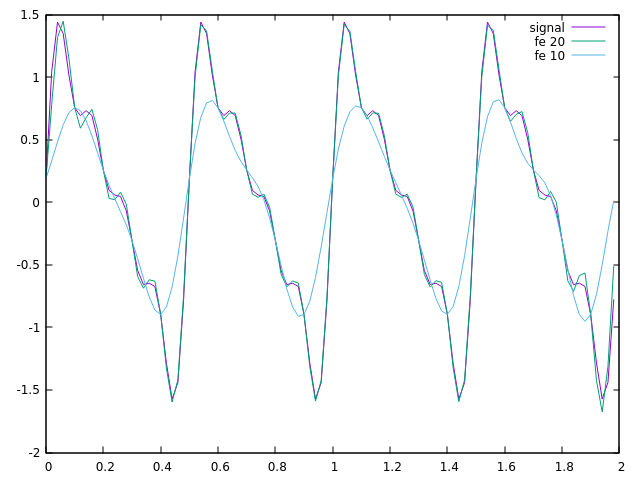
\includegraphics[scale=0.75]{Figures/Result.png}
\end{center}

\end{document}